\chapter{Introduction}

\section{Motivation}

Given the increase use of artificial intelligence solutions in reliably solving many of our current day-to-day problems, we decided to tackle the problem of face-based authentication in the systems that we use daily.

The challenge can be presented as follows: given a device that has access to a camera and which has been previously setup with a set of subject identities, the task is to validate the face in front of the camera as being known or not and in the positive case, the device should unlock itself.

The problems that arise are multiple and difficult to solve. Here are a few we focused on: firstly, the face in front of the camera should be validated as being real, therefore we need to give special attention to combating face spoofing attacks as printed photos, video replays or 3D masks. Secondly, the identification component of the system should be accurate enough so that two people with close facial features can be differentiated.

\begin{figure}[h]
	\begin{center}
		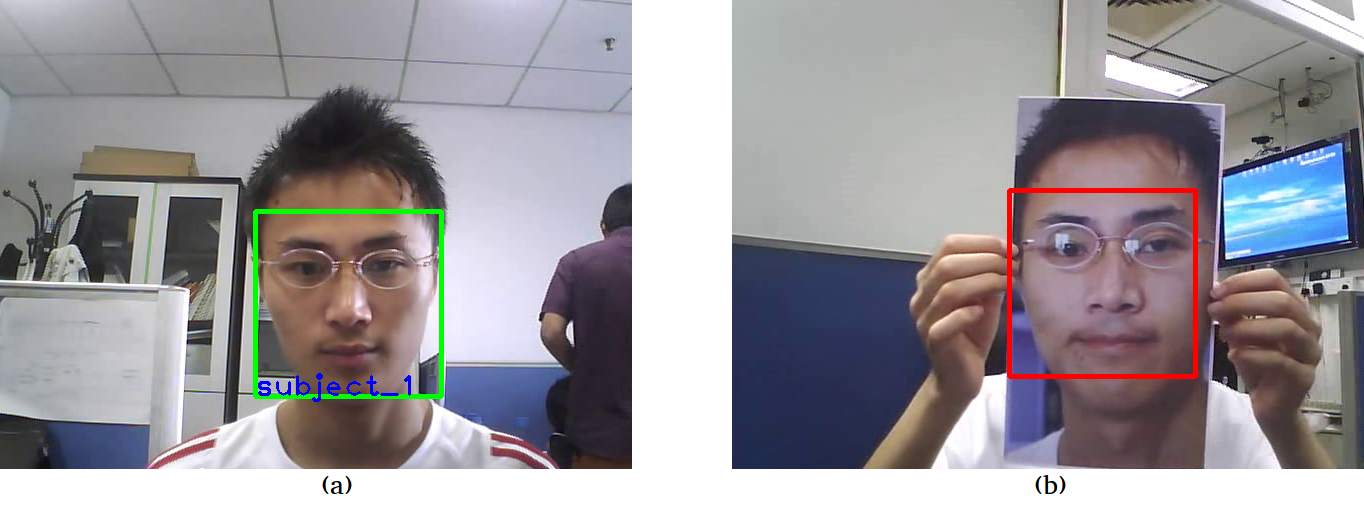
\includegraphics[width=15cm]{problem_representation}
		\caption[Desired behaviour of the face recognition system]{The face recognition system should validate the face as being real and then identify it (a) or in case it is an attack (b) - printed photo - should invalidate it}
	\end{center}
\end{figure}

\section{Impact}
A successful implementation of such a solution could be deployed to border control systems which would help amend the problem of crowded airports, could be used in the process of card payments as a method of reliable authentication and also could be used as an important part of an Artificial Intelligence assistant in order to create a more human-like experience.

\section{Thesis subject in the general context}
The first trials of developping facial recognition systems started out in the 1960s when Woodrow Bledsoe created a semi-automated system \cite{DavisMRETO64} containing a RAND tablet which was able to uniquely describe $10^{6}$ locations in a 10x10 inch area.
An operator was required to mark specific landmarks like the individual's  hairline, eyes and nose on this tablet and were used to calculate distances and rations to a point of reference and then compared to known data. The RAND tablet is considered to be the first graphical computer input device that is digital.

As the limits imposed by technology dropped and the potential in creating reliable facial recognition systems became worth taking into consideration, interest was shown by the Defense Advanced Research Products Agency (DARPA) which sponsored the Face Recognition Technology Evaluation (FERET) \cite{PhillipsJMHRSRP00} from 1993 to 1997 encouraging the development of face recognition algorithms and technologies by assessing the prototypes of face recognition systems. This project helped to a great extent to create a market of commercially available products.
Built upon the work of FERET, the Face Recognition Vendor Test \cite{PhillipsGMBTB03} developed by the National Institute of Standards and Technology \cite{FaceNist} along with DARPA and performed several times since 2000, it provides independent government evaluations of commercially available and prototype face recognition technologies and also helps identify future research direction for the face recognition scientific community.

We now present the results relative to one of the most reliable tests in the field. It based on the publicly available Labeled Faces in the Wild database. The current state of the art is held by deep learning approaches. We enlist some of the best results:
\begin{itemize}
	\item PingAn AI Lab with a mean accuracy of 0.9980 and std 0.0016
	\item Baidu with a mean accuracy of 0.9977 and std 0.0006
	\item FaceNet with a mean accuracy of 0.9963 and std 0.0016
\end{itemize}

\section{Structure of the thesis} 

\textbf{Chapter 2} contains four sections, each of them tackles an important stage of the entire pipeline in the application: 
\begin{itemize}
	\item \textbf{face detection} where we present the sliding window approach combined with histograms of oriented gradients (HOG) used to detect faces in an image
	\item \textbf{face alignment} where we show how to address the problem of facial landmark identification and positioning at a specific location in an image
	\item \textbf{face recognition} part where we introduce the neural network trained to learn a function that embeds a face image on an 128-dimensional euclidean space where the distance between two points corresponds to the similarities between the mapped faces
	\item \textbf{face validation} where we present the Local Binary Pattern, how to compute a feature descriptor based on it with the help of histograms and it's use in face validation
\end{itemize}

\textbf{In Chapter 3} we present our implementation of a face authentication system based on Python and on a powerful set of open-source tools as OpenCV\cite{opencv_library}, Scikit-learn\cite{scikit-learn}, Scikit-image\cite{scikit-image} and Openface\cite{amos2016openface}. These are well known frameworks and sustained both in the academically and industry fields. We create a command-line application consisting of the following pipeline that takes roughly $0.3$ seconds to iterate through:
\begin{itemize}
	\item capture an image from the laptop camera of size $480\times640$ using OpenCV
	\item detect the faces in the image using dlib face predictor that returns all face bounding boxes
	\item verify if they are live of spoof using our implementation of a face validator based on Local Binary Patterns and a Support Vector Machine with linear kernel
	\item compute the embedding of each face using the already trained Convolutional Neural Network of Openface
	\item recognize the faces by measuring the Euclidean distance between the embeddings of the detected faces and the ones already in the database
\end{itemize}

\textbf{In Chapter 4} we present the details of four databases that our face validation experiments are based on. We report the results for each of their evaluation protocols as well as a different cross-database evaluation in order to better simulate a real life use case. Additionally, we present another experiment in which we try to determine a threshold parameter for the face embedding function that is used in making the choice of whether two faces belong to the same identity.

Finally, we state the \textbf{conclusions} where we present our observations regarding the accuracy of local binary patterns in detecting spoof faces as well as the current results in terms of facial recognition systems based on deep learning methods with their reliableness.
